%!TEX root = Main.tex
\section{Tests}
Description of the tests made along with the procedures behind these test.

\subsection{Functionality test}

\subsection{Energy Test}

\section{Results}

Before the energy measurements are made, the functionality was validated. Using the test setup in section (fix me) a image was written to the flash, and then compress and send. 

\begin{figure}[H]
	\centering
	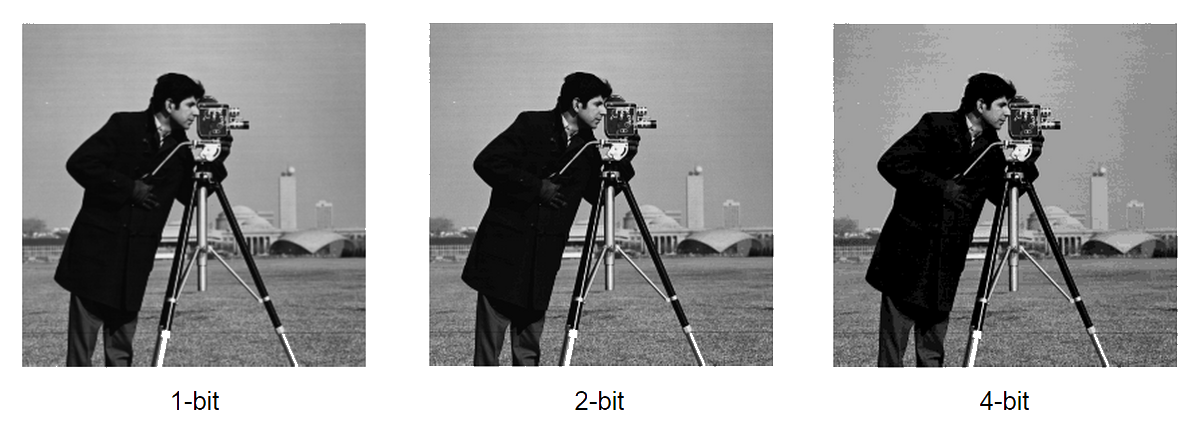
\includegraphics[width=0.8\textwidth] {cameramanresult}
	\caption{Compression Results}
	\label{fig:cameramanresult}
\end{figure}

The compressed images can be seen on figure \ref{fig:cameramanresult}. To ensure that the compression-send-decompress procedure was successful it is compared with the same image compressed and decompressed in Matlab. By comparing this two images it is shown that the functionality is as expected. 


Looking at the voltage over the shunt, we can see how the system uses power, for the test setup a typical power over time is illustrated in figure \ref{fig:ImageTransfere}

\begin{figure}[H]
	\centering
	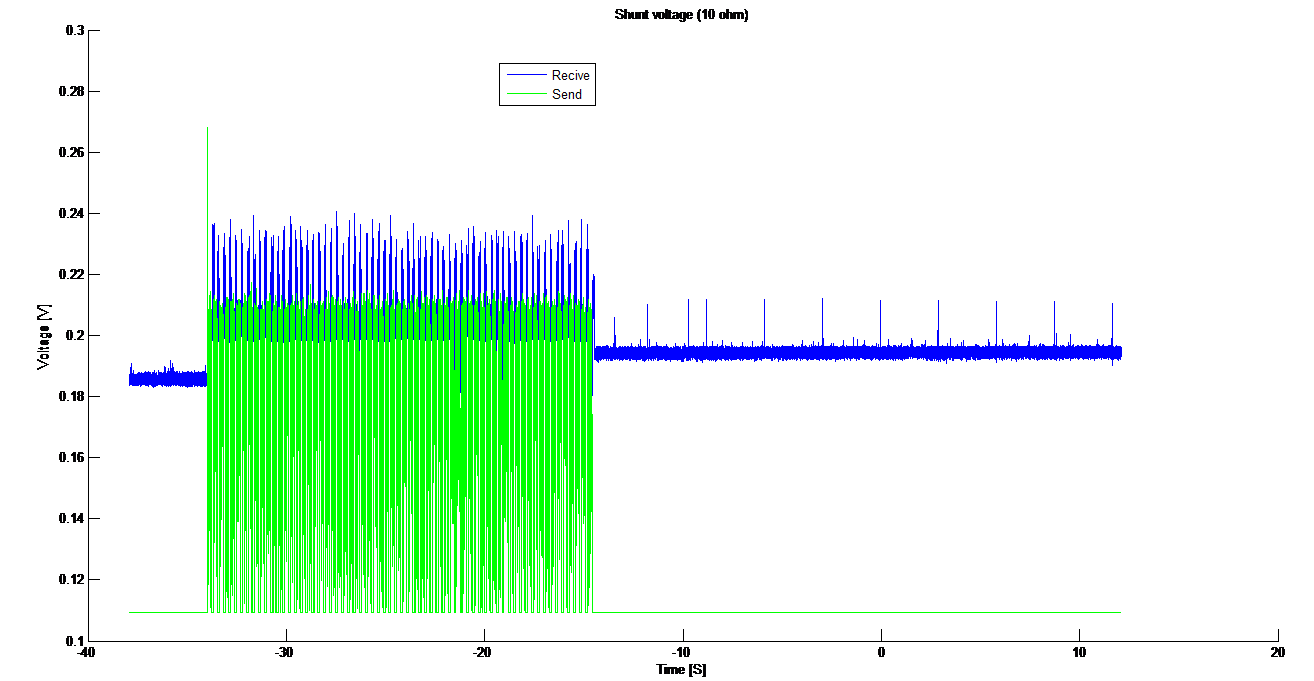
\includegraphics[width=1\textwidth ]{ImageTransfere}
	\caption{ Shut voltage during image transfer. }
	\label{fig:ImageTransfere}
\end{figure}

For each compression algorithm 3 measurements was done on both sender and receiver. The measurements can be seen in the table \ref{tab:MeasurementResults} 

 

\begin{table}[h]
\begin{tabular}{c|l|l|l|l|ll}
\cline{2-5}
\multicolumn{1}{l|}{}                       & \multicolumn{2}{l|}{Energy {[}J{]}} & \multicolumn{2}{l|}{Mean Power {[}W{]}} &                                            &                                             \\ \hline
\multicolumn{1}{|l|}{Bit Removed}           & Recive           & Send             & Recive             & Sender             & \multicolumn{1}{l|}{Transfer Time {[}S{]}} & \multicolumn{1}{l|}{Better Power Than None} \\ \hline
\multicolumn{1}{|c|}{\multirow{3}{*}{None}} & 14,638           & 14,405           & 0,639              & 0,626              & \multicolumn{1}{l|}{23,0}                  & \multicolumn{1}{l|}{0\%}                    \\ \cline{2-7} 
\multicolumn{1}{|c|}{}                      & 14,666           & 14,432           & 0,639              & 0,626              & \multicolumn{1}{l|}{23,0}                  & \multicolumn{1}{l|}{0\%}                    \\ \cline{2-7} 
\multicolumn{1}{|c|}{}                      & 14,609           & 14,385           & 0,639              & 0,626              & \multicolumn{1}{l|}{23,0}                  & \multicolumn{1}{l|}{0\%}                    \\ \hline
\multicolumn{1}{|c|}{\multirow{3}{*}{One}}  & 13,527           & 13,248           & 0,642              & 0,625              & \multicolumn{1}{l|}{21,2}                  & \multicolumn{1}{l|}{8\%}                    \\ \cline{2-7} 
\multicolumn{1}{|c|}{}                      & 13,535           & 13,252           & 0,642              & 0,626              & \multicolumn{1}{l|}{21,2}                  & \multicolumn{1}{l|}{8\%}                    \\ \cline{2-7} 
\multicolumn{1}{|c|}{}                      & 13,528           & 13,254           & 0,642              & 0,625              & \multicolumn{1}{l|}{21,2}                  & \multicolumn{1}{l|}{8\%}                    \\ \hline
\multicolumn{1}{|c|}{\multirow{3}{*}{Two}}  & 12,469           & 12,189           & 0,643              & 0,625              & \multicolumn{1}{l|}{19,5}                  & \multicolumn{1}{l|}{15\%}                   \\ \cline{2-7} 
\multicolumn{1}{|c|}{}                      & 12,477           & 12,206           & 0,643              & 0,626              & \multicolumn{1}{l|}{19,5}                  & \multicolumn{1}{l|}{15\%}                   \\ \cline{2-7} 
\multicolumn{1}{|c|}{}                      & 12,467           & 12,190           & 0,643              & 0,625              & \multicolumn{1}{l|}{19,5}                  & \multicolumn{1}{l|}{15\%}                   \\ \hline
\multicolumn{1}{|c|}{\multirow{3}{*}{Four}} & 9,566            & 9,317            & 0,646              & 0,624              & \multicolumn{1}{l|}{14,9}                  & \multicolumn{1}{l|}{35\%}                   \\ \cline{2-7} 
\multicolumn{1}{|c|}{}                      & 9,556            & 9,309            & 0,646              & 0,625              & \multicolumn{1}{l|}{14,9}                  & \multicolumn{1}{l|}{35\%}                   \\ \cline{2-7} 
\multicolumn{1}{|c|}{}                      & 9,533            & 9,298            & 0,644              & 0,625              & \multicolumn{1}{l|}{14,9}                  & \multicolumn{1}{l|}{35\%}                   \\ \hline
\end{tabular}
\caption{Measurement Results }
\label{tab:MeasurementResults}
\end{table}

